%!TEX root = ../bachelorthesis.tex
\chapter{Implementierung}
\label{chap:implementierung}
Nachdem der grundsätzliche Aufbau und Ablauf der Kommunikation des Gesamtprogramms beschrieben wurde, werden nun die Details der einzelnen Module dargestellt.

\section{Moveit Path Planning Node} % (fold)
\label{sec:universal_robot_impl}

An diesem Programm wurden einige Anpassungen vorgenommen. Zum einen wurde die in MoveIt! benutzte Bibliothek zur Lösung der inversen Kinematik KDL durch TRAC\_IK ausgetauscht. Diese Bibliothek wird dazu verwendet, für eine gewünschte Position und Orientierung des Roboterarms die dazu erforderlichen Winkel der Gelenke zu berechnen. Während der Versuche war es teilweise zu beobachten, dass MoveIt! keinen oder nur einen viel zu komplizierten Weg von der Start- zur Zielkonfiguration gefunden hat. Dieses Problem konnte teilweise durch diesen Austausch mit TRAC\_IK behoben werden.

Zusätzlich wurde das URDF in diesem Paket angepasst. Das URDF enthält die geometrischen Informationen über den Roboterarm, wie z.B. die Länge und Form der einzelnen Glieder und die Position der Werkzeugaufnahme des Arms. Wird dem Arm eine Zielposition und Orientierung übergeben, so gilt diese normalerweise für diese Werkzeugaufnahme. Für die Bachelorarbeit wurde jedoch das Kalibrierungsmuster an diese Stelle montiert. Das Muster wurde nicht mittig an der Werkzeugaufnahme angebracht, sondern steht seitlich ab. Daher wurde im URDF der Endpunkt des Arms von der Werkzeugaufnahme auf den Mittelpunkt des Kalibrierungsmusters versetzt. Das führt dazu, dass sich nun nicht mehr die Werkzeugaufnahme des Arms an der Zielposition befindet, sondern der Mittelpunkt des Kalibrierungsmusters.
\todo{Foto vom Caltab am Endeffector}

\section{Client Side Path Planning Node} % (fold)
\label{sec:movearmserver_impl}
Diese Node wurde in der Programmiersprache Python entwickelt und hat den Namen \texttt{MovementHandler.py}. Sie hat den Auftrag, die Bewegung des Arms zu koordinieren und dazu mit MoveIt! zu kommunizieren.

Das Programm erhält beim Start die Position der Kamera in Relation zur Basis des Arms. Außerdem wird ein Actionserver gestartet, der auf Aufgaben vom Typ \texttt{move\_arm} wartet. Zusätzlich wird der Kommunikationskanal zu MoveIt! gestartet.

Die Aufgabe \texttt{move\_arm} ermöglicht es einem Actionclient, den Roboterarm zu einer von ihm gewählten Position zu bewegen. Zusätzlich kann er die horizontale und vertikale Neigung des Musters bestimmen.

Erhält das Programm eine Aufgabe, so wird zunächst für die gewünschte Position die Orientierung des Arms berechnet. Dazu wird zunächst angenommen, dass das Kalibrierungsmuster orthogonal zur Kamera stehen soll. Jede Position lässt sich mit den drei Variablen $x, y, z$ definieren. Dadurch lässt sich jede Position auch als Ortsvektor darstellen:
\begin{equation}
	\vec{p} = 
	\begin{pmatrix}
		x\\
		y\\
		z
	\end{pmatrix}
\end{equation}

Um nun die Orientierung zu errechnen, subtrahiert man zunächst den Vektor für die Position der Kamera vom Vektor für die Position des Roboterarms. Der daraus resultierende Vektor $\vec{p}_{diff}$ beschreibt die geometrische Transformation vom Arm zur Kamera. 
\begin{equation}\label{eq:diff}
	\vec{p}_{Diff} = \vec{p}_{Roboter} - \vec{p}_{Kamera}
\end{equation}
Mit diesem Vektor lässt sich nun der Gierwinkel $\alpha$ und Neigungswinkel $\beta$ bestimmen, damit das Muster orthogonal zur Kamera steht:
\begin{equation}\label{eq:pitch}
	\alpha = \arctantwo(y_{diff}, x_{diff})
\end{equation}
\begin{equation}\label{eq:yaw}
	\beta = -\arcsin(x_{diff})
\end{equation}

Mit diesen Winkeln würde nun das Muster orthogonal zur Kamera zeigen. Wurden in der Aufgabe zusätzliche Neigungen angegeben, werden diese nun zu diesen Winkeln addiert.

Schließlich muss noch der Rollwinkel $\gamma$ bestimmt werden. In diesem Anwendungsfall soll das Kalibrierungsmuster immer nach außen zeigen und parallel zum Boden stehen, damit die Reichweite des Roboters erhöht wird. Dazu wird die folgende Gleichung gelöst:
\begin{equation}
	\gamma = \arctantwo(y_{Roboter}, x_{Roboter}) - \arctantwo(y_{Kamera}, x_{Kamera})
\end{equation}
Ist $\gamma > 0$, so befindet sich das Muster von der Kamera aus gesehen in der rechten Hälfte des Bildes. Damit das Muster nach außen zeigt, muss der Rollwinkel 0$^\circ$ betragen. Ist $\gamma < 0$, befindet sich das Muster in der linken Hälfte und der Rollwinkel wird auf 180$^\circ$ gesetzt.

Wurde die Orientierung berechnet, muss für die Position und Orientierung ein Plan generiert werden, mit dem sich der Arm aus der Startposition zur Zielposition bewegt, ohne dass er mit sich selbst oder der Umgebung kollidiert. Diese Aufgabe übernimmt MoveIt!. Aufgrund des eingesetzten Algorithmus in MoveIt! können für gleiche Start- und Zielpositionen unterschiedliche Pläne erstellt werden, teilweise kann MoveIt! auch keinen Plan finden. Daher werden für jede Aufgabe, die der Actionserver erhält, fünf Pläne von MoveIt! erzeugt. Wenn die gewünschte Position nicht erreichbar ist oder Teile des Roboters oder das Kalibrierungsmuster mit sich selber oder der Umgebung kollidieren würden, sind alle fünf Pläne leer. In diesem Fall wird die Aufgabe abgebrochen und dem Actionclient eine negative Rückmeldung zurückgegeben. Ansonsten wird der Plan ausgewählt, der die geringste Anzahl an Zwischenpositionen enthält, und an MoveIt! zur Ausführung übermittelt. Hat MoveIt! die erfolgreiche Ausführung bestätigt, wird dem Actionclient die Aufgabe positiv bestätigt.

\section{Computer Vision Node} % (fold)
\label{sec:caltab_detector_node_impl}
Diese Node wurde in der Programmiersprache C++ programmiert und liegt im Paket \texttt{caltab\_detector} mit dem Dateinamen \texttt{caltab\_detector\_node.cpp}. Sie dient dazu, die von der Kamera übermittelten Bilder auszuwerten und zur Kalibrierung vorzuhalten.

Vor dem Start muss der Benutzer über die Datei \texttt{caltab\_detector/config/parameters.yaml} einige Parameter konfigurieren. Diese sind in \autoref{tab:caltab_detector} aufgeführt.

\begin{table}
\begin{tabularx}{\textwidth}{|l|X|}
	\hline
	Parametername & Beschreibung \\\hline
	focal\_length & Brennweite in Metern \\\hline
	sensor\_size x & Größe des Sensors entlang der x-Achse in Metern \\\hline
	sensor\_size y & Größe des Sensors entlang der y-Achse in Metern \\\hline
	resolution x & Anzahl der Pixel des Bildes entlang der x-Achse \\\hline
	resolution y & Anzahl der Pixel des Bildes entlang der y-Achse \\\hline
	image\_topic & Der Name des Topics, auf dem die Bilder von der Kamera veröffentlicht werden \\\hline
	description\_file & Der Pfad zu der Datei, die die Beschreibung für das Kalibrierungsmuster enthält \\\hline
\end{tabularx}
\caption{Beschreibung der Parameter für die Computer Vision Node}
\label{tab:caltab_detector}
\end{table}

Über das angegebene Topic erhält das Programm die Bilder der Webcam. Zusätzlich stellt das Programm zwei Actionserver zur Verfügung. Der Actionserver mit dem Namen \texttt{find\_calibration\_object} hat die Aufgabe, in dem aktuellen Bild der Webcam nach dem Kalibrierungsmuster zu suchen. Der Actionclient kann für jeden Auftrag angeben, in wie vielen aufeinanderfolgenden Bildern der Server nach dem Muster suchen soll, da dieses nicht immer im ersten Versuch gefunden wird. Hat der Server das Muster innerhalb der erlaubten Anzahl von Bildern gefunden, erhält der Client eine positive Rückmeldung, ansonsten eine negative.

Der zweite Actionserver \texttt{Calibrate} führt die Kalibrierung durch und errechnet aus allen Bildern, in denen das Muster zu sehen war, die intrinsischen Parameter, die Verzeichnungsparameter und den mittleren Fehler. Zusätzlich werden diese Bilder auf der Festplatte abgespeichert. Für jedes Bild wird außerdem eine Kopie angefertigt, in der eine Simulation des Musters über das im Bild zu sehende Muster gelegt wird. Dadurch kann zusätzlich visuell die Qualität der Kalibrierung überprüft werden.

Beim Start der Node kann der Benutzer ein Verzeichnis angeben, in dem die Bilder gespeichert werden sollen. Andernfalls wird in dem aktuellen Verzeichnis ein Unterordner erstellt. Außerdem wird die Datei gelesen, in der die initialen intrinsischen Parameter für die eingesetzte Kamera hinterlegt sind. Ebenfalls wird die Datei gelesen, in der die Dimensionen und Eigenschaften des benutzten Kalibrierungsmusters definiert sind. Anschließend verbindet sich das Programm mit dem Topic der Kamera, um die Bilder zu empfangen.

Jedes Mal, wenn das Programm ein aktuelles Bild von der Kamera erhält, wird die Methode \texttt{subscriberCallback} aufgerufen. Die Methode überprüft zunächst, ob auf Grund eines laufenden Auftrags für den find\_calibration\_object Actionserver noch Bilder überprüft werden sollen. Ist dies nicht der Fall, wird die Methode direkt beendet und das Programm wartet weiter auf eingehende Aufträge oder neue Bilder. 

Wenn jedoch ein Auftrag aktiv ist und das aktuelle Bild ausgewertet werden soll, wird die Methode weiter abgearbeitet. Das empfangene Bild ist vom Typ \texttt{sensor\_msgs::Image}. Um es aber mit HALCON benutzen zu können, muss es zu dem Typ \texttt{HObject} umgewandelt werden. Dazu wird das Bild in einem Zwischenschritt mit Hilfe der Methode \texttt{toCvCopy} aus dem Paket \texttt{cv\_bridge} in ein Objekt vom Typ \texttt{cv::Mat} konvertiert. Dadurch kann man nun relativ einfach auf den Wert für jedes einzelne Pixel zugreifen. Anschließend wird Pixel für Pixel über das gesamte Bild iteriert und die Werte der Pixel werden in einem \texttt{unsigned char*} gespeichert. Die HALCON-Methode \texttt{GenImage1} liest dann die Werte aus dem \texttt{unsigned char*} und erstellt das \texttt{HObject}.

Für jedes auszuwertende Bild wird ein fortlaufender Index erstellt, der im weiteren Verlauf benötigt wird. Es wird nun die HALCON-Methode \texttt{FindCalibObject} aufgerufen. Diese sucht in dem eben erstellten Bild nach dem Kalibrierungsmuster. Wird das Muster nicht erkannt, wirft diese Methode eine Exception. Diese wird im weiteren Verlauf der \texttt{subscriberCallback}-Methode gefangen und in der Konsole wird die Fehlermeldung von HALCON ausgegeben. Kann HALCON das Muster erkennen, wird es intern unter dem Index abgespeichert und zusätzlich in dem vom Benutzer angegeben Ordner gespeichert. In einer von diesem Programm verwalteten Liste wird zusätzlich der Index dieses Bildes abgespeichert. Der boolesche Wert caltabFound wird auf wahr gesetzt und die Anzahl der noch auszuwertenden Bilder für den aktuellen Auftrag auf null. 

Erhält der find\_calibration\_object Actionserver einen neuen Auftrag, wird die Methode \texttt{find\_calibration\_objectAction} aufgerufen. Zunächst wird der boolesche Wert auf falsch und die Anzahl der auszuwertenden Bilder auf den Wert gesetzt, der im Auftrag vom Client angegeben wurde. Dann wartet die Methode so lange, bis entweder die angegebene Anzahl an Bildern ausgewertet wurde oder vorher ein Kalibrierungsmuster gefunden wurde. Ist der boolesche Wert caltabFound wahr, wird dem Client eine positive Rückmeldung gegeben, sonst eine negative.

Wenn der Calibrate Actionserver einen Auftrag erhält, wird die Kalibrierung durchgeführt. Dazu wird zunächst die HALCON-Methode \texttt{CalibrateCameras} aufgerufen. Diese berechnet intern die neuen intrinsischen Parameter und die Parameter für die Verzeichnung. Außerdem wird der mittlere Fehler zurückgegeben. Um nun die neuen Parameter zu erhalten, wird die HALCON-Methode \texttt{GetCalibData} aufgerufen. Die so erhaltenen Werte werden zunächst in Werte vom Typ \texttt{double} umgewandelt. Dann werden dem Client diese Werte, der Fehler und die Anzahl der zur Kalibrierung benutzten Bilder zurückgegeben.

Anschließend wird nacheinander jedes abgespeicherte Bild mit Hilfe der Liste, die alle Indizes enthält, noch einmal mit HALCON eingelesen. Zunächst wird für das Bild die Position und Orientierung des Kalibrierungsmuster von HALCON ausgelesen, wie es von HALCON erkannt wurde. Dann werden diese Informationen mit den neuen Kameraparametern korrigiert. Schließlich wird das so korrigierte Kalibrierungsmuster über das eingelesene Bild gelegt und das Bild so auf dem Dateisystem abgespeichert. Siehe dazu \autoref{img:example_caltab} und \autoref{img:example_caltab_added}.
\begin{figure}
\centering
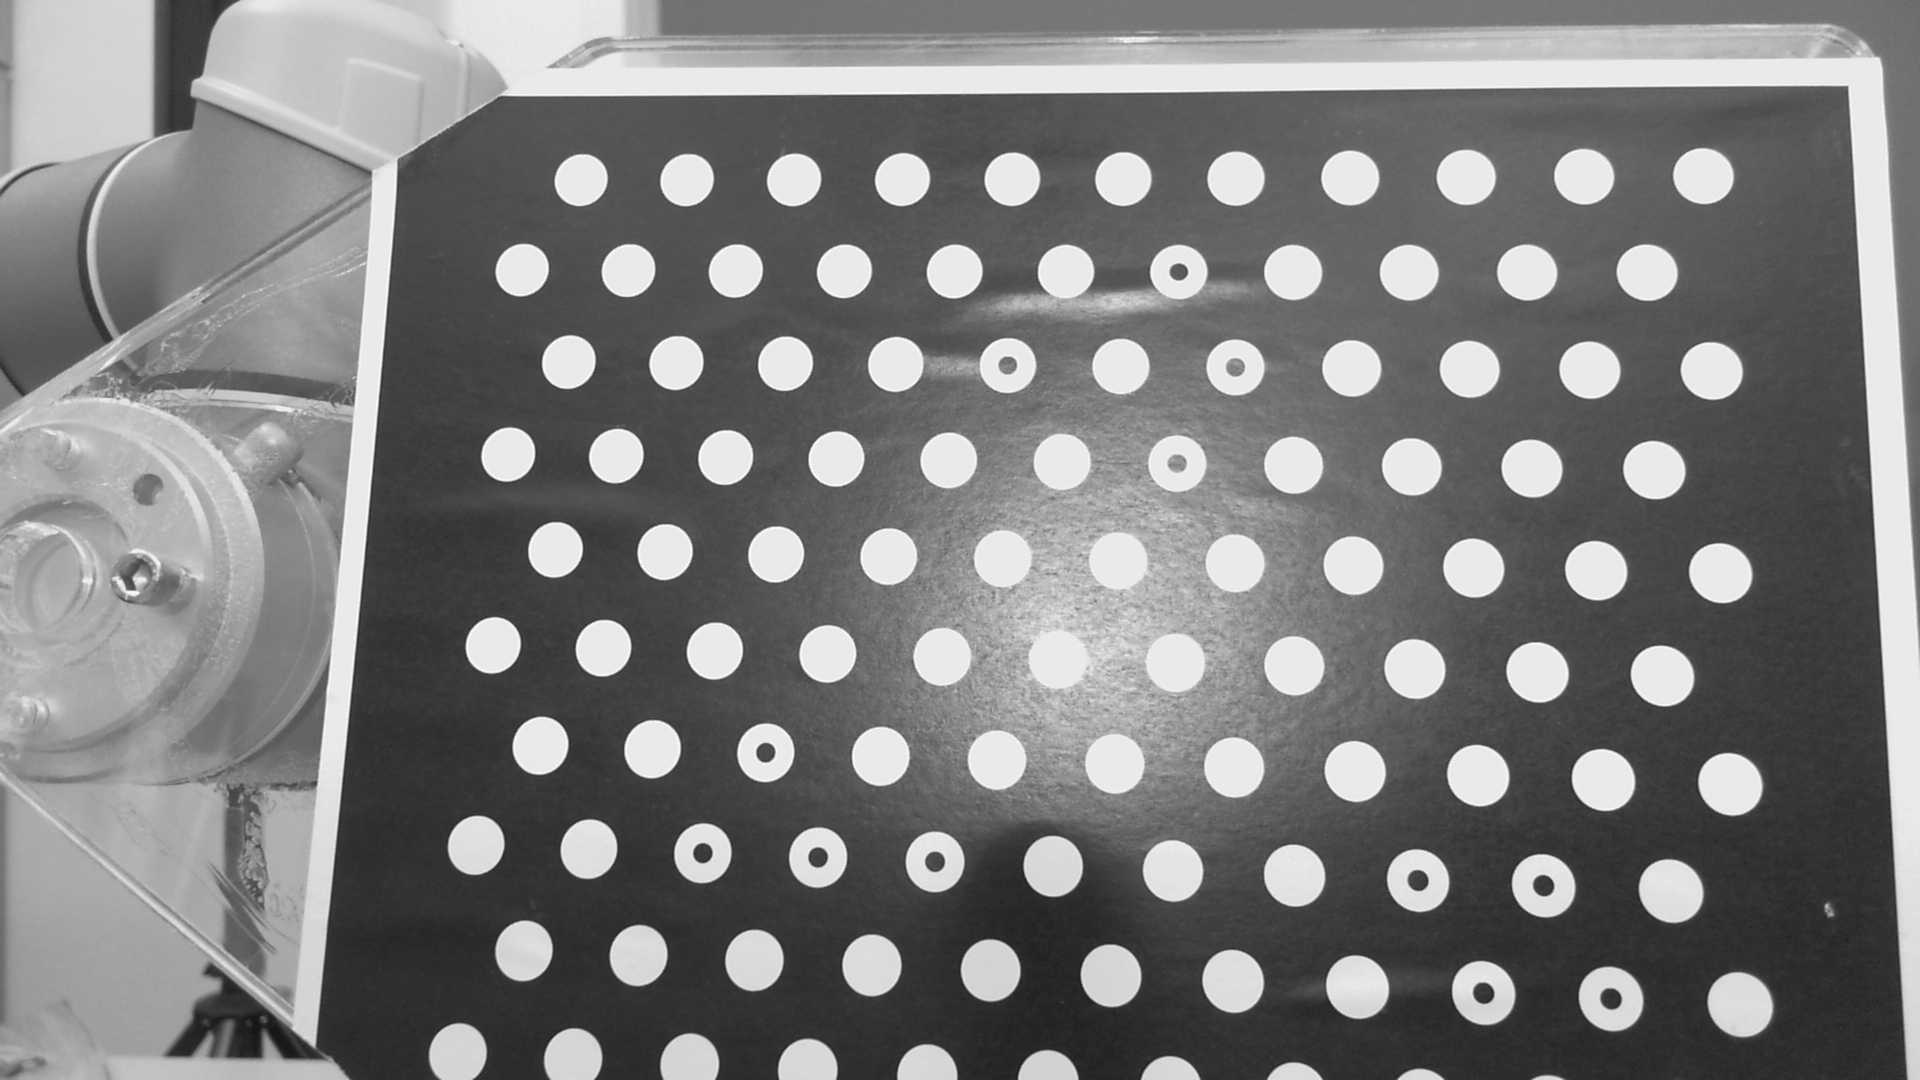
\includegraphics[width=\textwidth]{images/example_caltab}
\caption{Das Originalbild.}\label{img:example_caltab}
\end{figure}
\begin{figure}
\centering
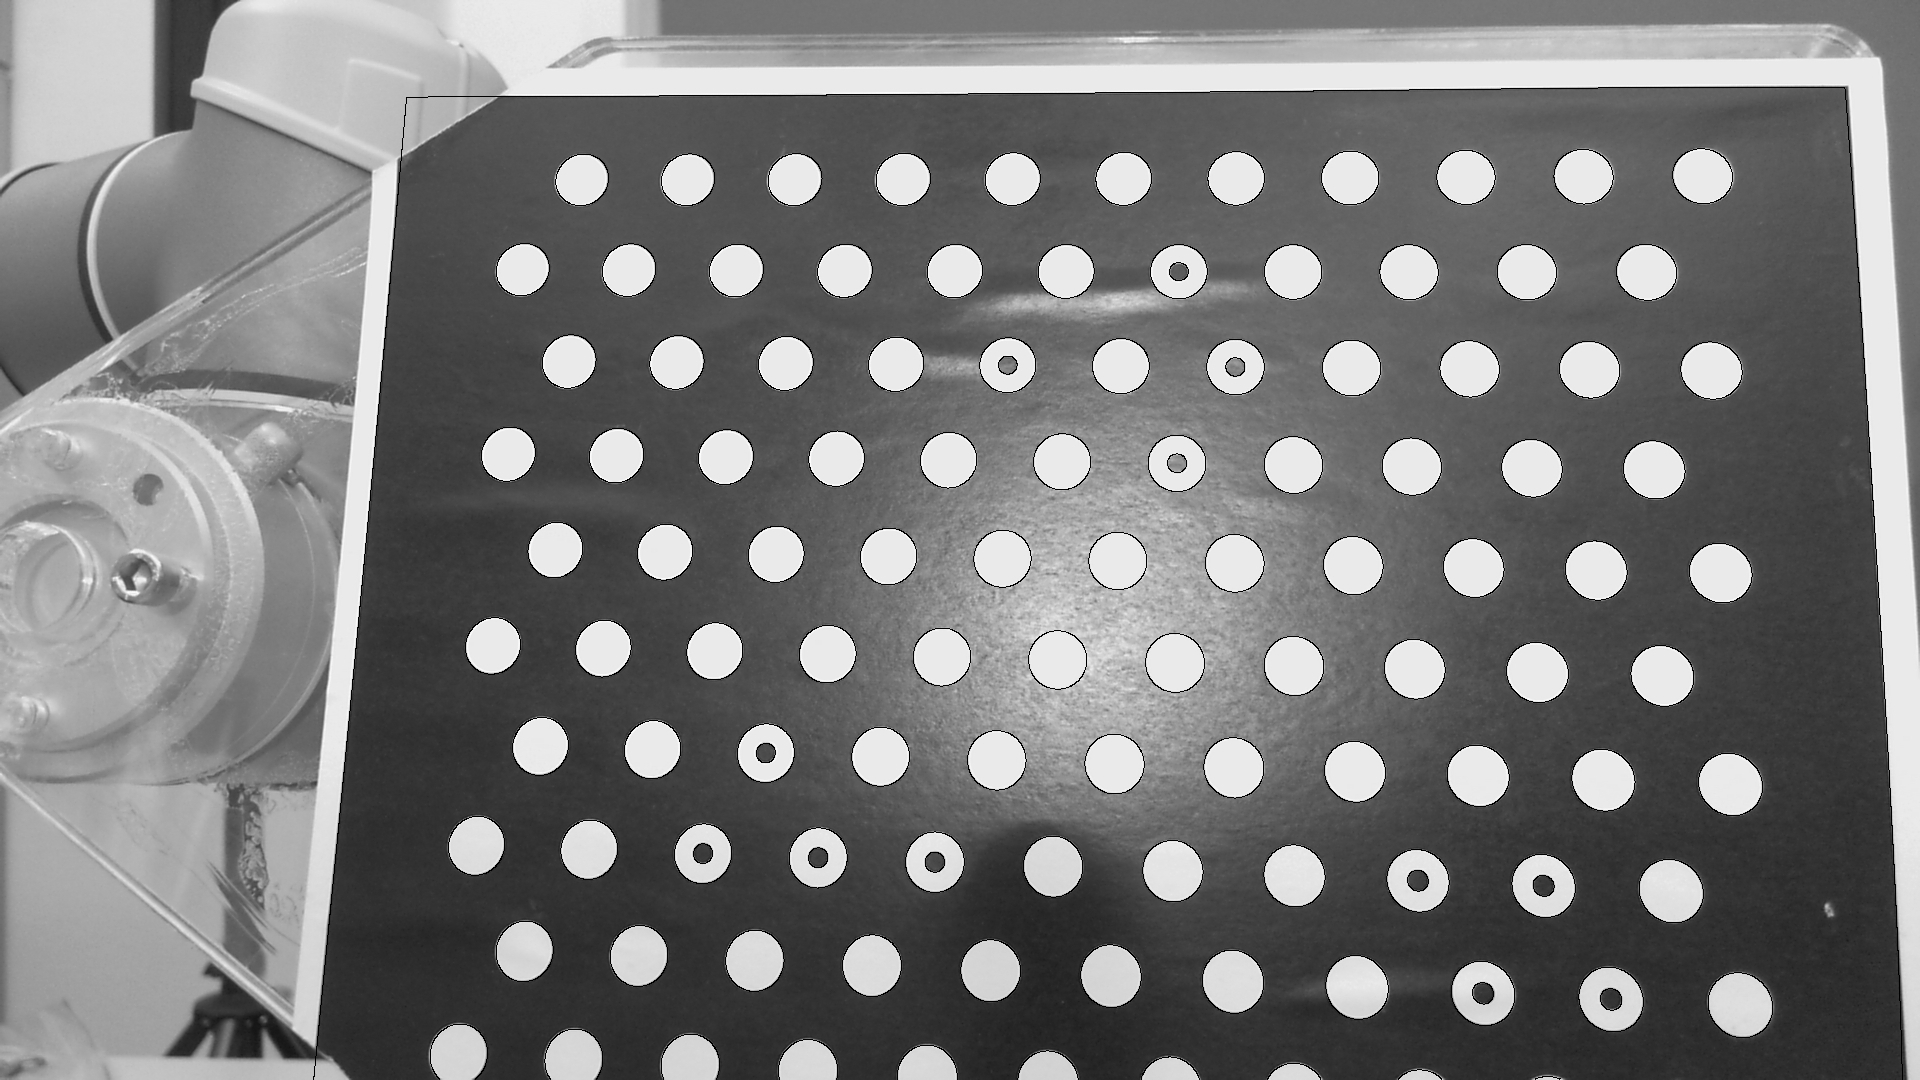
\includegraphics[width=\textwidth]{images/example_caltab_added}
\caption{Das Bild mit dem eingezeichneten Kalibrierungsmuster. Man beachte die feinen Linien, die um das schwarze Rechteck und in die Kreise eingefügt wurden.}\label{img:example_caltab_added}
\end{figure}

\section{MovementController} % (fold)
\label{sec:movementcontroller_impl}
Die Klasse MovementController wurde wieder in Python entwickelt. Sie agiert als Actionclient für den move\_arm Actionserver und den find\_calibration\_object Actionserver und koordiniert die Bewegung des Arms zu den verschiedenen Positionen und die anschließende Suche nach dem Kalibrierungsmuster im Bild. Sie wird vom High Level Executive gestartet.

Beim Start der Klasse über den \texttt{CalibrationController} kann ihr als Argument durch den Benutzer eine Verzögerung in Sekunden übergeben werden. Dies hat den Hintergrund, dass einige Kamerasensoren eine nicht unerhebliche Verzögerung zwischen der Bildaufnahme und dem Veröffentlichen über einen Topic aufweisen. Bei einer zu geringen Verzögerung zwischen dem Erreichen der Position und der Auswertung der Bilder kann der Arm auf den Bildern noch in Bewegung sein. Dadurch wird das Muster entweder an der falschen Stelle ausgewertet oder es ist so unscharf abgebildet, dass es nicht erkannt werden kann.

Die Klasse führt nach ihrer Initialisierung nichts weiter aus, sondern stellt dem \texttt{High Level Executive} die Methode \texttt{execute\_different\_orientations} zur Verfügung. Dieser Methode muss eine Position übergeben werden, an die das Kalibrierungsmuster bewegt werden soll. Für diese Position wird dann zunächst ein Bild ohne zusätzliche Neigung gemacht. Anschließend wird das Bild in 10$^\circ$-Schritten nach oben, unten, links und rechts geneigt, wobei für jede Orientierung wieder ein Bild aufgenommen wird. Dazu ruft der \texttt{MovementController} die Methode \texttt{take\_picture\_with\_orientation} auf. Dieser Methode wird ebenfalls die Position übergeben und zusätzlich die gewünschte horizontale und vertikale Neigung. Zunächst wird also diese Methode ohne zusätzliche Neigung aufgerufen, anschließend mit den unterschiedlichen Varianten.

Die \texttt{take\_picture\_with\_orientation}-Methode schickt zunächst an den move\_arm Actionserver einen neuen Auftrag mit der übergebenen Position und Orientierung. Anschließend wartet sie auf die Rückmeldung vom Server. Ist diese negativ, gibt sie auch der Methode \texttt{execute\_different\_orientations}, die sie aufgerufen hat, eine negative Rückmeldung. Wenn der Arm erfolgreich an die gewünschte Position bewegt wurde, wartet sie die konfigurierte Zeit ab, bis sie dem find\_calibration\_object Actionserver einen Auftrag schickt, um in den neusten Bildern nach dem Kalibrierungsmuster zu suchen. Die Rückmeldung von diesem Server ist wieder dafür ausschlaggebend, ob die Methode eine positive oder negative Rückmeldung zurückgibt.

Wenn der Aufruf der \texttt{take\_picture\_with\_orientation}-Methode ohne zusätzliche Neigung fehlschlägt, werden die unterschiedlichen Neigungen übersprungen. Dies passiert entweder, wenn die Position nicht vom Roboter erreicht werden kann, oder ein Fehler an einem anderen Teil der Software auftritt.

Nachdem die \texttt{execute\_different\_orientations}-Methode alle unterschiedlichen Orientierungen durchgegangen oder bereits an der ersten Position gescheitert ist, gibt sie die Anzahl der Bilder zurück, in denen das Muster gefunden wurde.

\section{High Level Executive} % (fold)
\label{sec:calibrationcontroller_impl}
Diese Klasse wurde auch in Python entwickelt. Sie errechnet die verschiedenen Positionen, an die das Kalibrierungsmuster bewegt werden soll, übergibt diese nacheinander an den \texttt{MovementController} und ruft zum Schluss den Calibrate Actionserver auf.

Beim Aufruf dieser Klasse müssen ihr mehrere Parameter übergeben werden. Diese werden in der Datei \texttt{robot\_assisted\_calibration/config/parameters.yaml} definiert, siehe \autoref{tab:high_level_executive}

\begin{table}
\begin{tabularx}{\textwidth}{|l|X|}
	\hline
	Parametername & Beschreibung \\\hline
	close\_distance\_factor & Der Faktor, der die kurze Entfernung bestimmt \\\hline
	medium\_distance\_factor & Der Faktor, der die mittlere Entfernung bestimmt \\\hline
	far\_distance\_factor & Der Faktor, der die weite Entfernung bestimmt \\\hline
	focal\_length & Brennweite in Metern \\\hline
	sensor\_size x & Größe des Sensors entlang der x-Achse in Metern \\\hline
	sensor\_size y & Größe des Sensors entlang der y-Achse in Metern \\\hline
	calibration\_object\_height & Die Höhe des Kalibrierungsmusters in Metern \\\hline
	calibration\_object\_width & Die Breite des Kalibrierungsmusters in Metern \\\hline
	camera\_position & Die Position der Kamera in Relation zur Basis des Roboters \\\hline
	skip\_orientations & zu Testzwecken kann dieser Parameter auf true gesetzt werden, um die zusätzlichen Orientierungen zu überspringen \\\hline
\end{tabularx}
\caption{Beschreibung der Parameter für den High Level Executive}
\label{tab:high_level_executive}
\end{table}

Die Entfernung des Musters zur Kamera wird nicht absolut angegeben. Stattdessen wird die Höhe des Musters im Bild zur Entfernungsbestimmung benutzt. Die Entfernung, bei der die Höhe des Musters im Bild 80\% der gesamten Bildhöhe ausmacht, ist die kurze Entfernung. Bei der mittleren Entfernung beträgt die Höhe des Musters 50\%. Bei der weiten Entfernung sind es nur noch 30\%. Je nach Sensorgröße und Brennweite sind diese Werte allerdings nicht geeignet; die Entfernungen könnten zu nah beieinander liegen oder aber sie sind so groß, dass die Positionen nicht mehr für den Arm erreichbar sind. In diesen Fällen müssen die Faktoren an die Situation angepasst werden.

Bei der Initialisierung wird zunächst ein Objekt vom Typ \texttt{MovementController} erstellt. Danach folgt die Bestimmung der Positionen für das Kalibrierungsmuster.

Dazu werden im ersten Schritt die drei unterschiedlichen Entfernungen des Musters zur Kamera benötigt. Dies geschieht mit der folgenden Formel. $h_{Muster}$ definiert die Höhe des Musters in Metern, $h_{Sensor}$ die Höhe des Sensors in Metern, $f$ die Brennweite in Metern und der Faktor definiert, wie hoch das Muster im Bild sein soll. Das Ergebnis $d$ ist ebenfalls in Metern.
\begin{equation}
	d = \frac{h_{Muster} \times f }{h_{Sensor} \times factor}
\end{equation}
In diese Formel werden die oben genannten Werte eingesetzt, also im Standardfall 0,8 , 0,5 und 0,3.

Nun kann die Position mit der kurzen Distanz bestimmt werden. Diese besteht aus den Koordinaten $\begin{pmatrix}
	d\\ 0\\ 0
\end{pmatrix}$, da das Muster mittig vor der Kamera mit der soeben berechneten Distanz zu sehen seien soll.

Die anderen Positionen sind aufwändiger zu bestimmen, da bis auf eine alle anderen nicht zentriert vor der Kamera sind. Für die mittlere Distanz $d$ wird jetzt berechnet, wie hoch und breit das Sichtfeld ist. Dazu werden die folgenden Formeln benutzt. Alle Werte sind in Metern.
\begin{equation}\label{eq:fov-height}
	h_{Sichtfeld} = \frac{h_{Sensor} \times d}{f}
\end{equation}
\begin{equation}\label{eq:fov-width}
	b_{Sichtfeld} = \frac{b_{Sensor} \times d}{f}
\end{equation}
Nun ist bekannt, wie groß das Sichtfeld zu dieser Distanz ist. Das Muster soll sich in jedem Quadrant des Bildes befinden. Eine Position wird beispielhaft für den Quadranten oben links gezeigt.
\begin{equation}\label{eq:position}
	\begin{pmatrix}
		d\\
		-b_{Sichtfeld} / 2 - b_{Muster} / 2\\
		h_{Sichtfeld} / 2 - h_{Muster} / 2
	\end{pmatrix}
\end{equation}
Die weiteren Positionen für diese Distanz werden durch das Hinzufügen oder Weglassen der Vorzeichen bestimmt.

Die Berechnung der Positionen für die lange Distanz wird analog dazu durchgeführt. Das Bild wird in diesem Fall jedoch nicht in vier sondern neun Bereiche aufgeteilt. Zunächst wird wieder das Sichtfeld bestimmt, siehe \autoref{eq:fov-height} und \autoref{eq:fov-width}. Die Positionen in den Ecken werden genau so wie in \autoref{eq:position} bestimmt. Für die Positionen, die auf einer der Achsen liegen, wird der entsprechende y- oder z-Wert auf null gesetzt.

Eine Übersicht über die verschiedenen Positionen sieht man in \autoref{img:marker_side}.
\begin{figure}
\centering
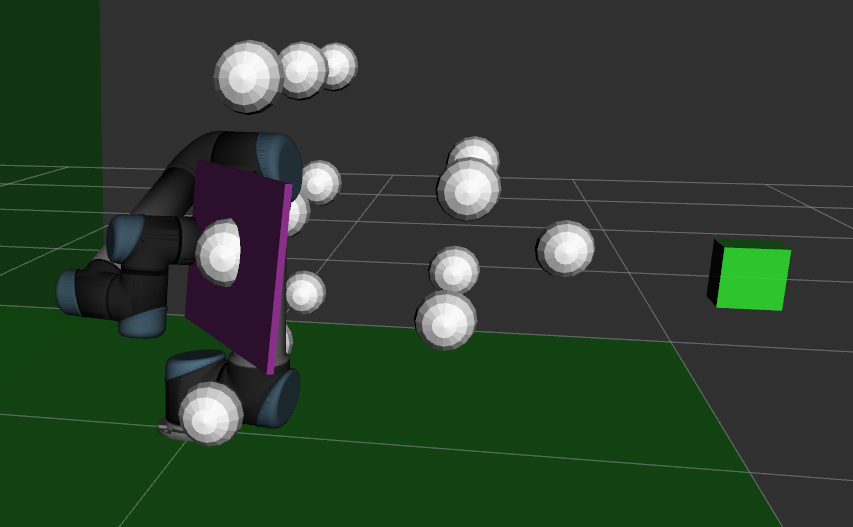
\includegraphics[width=\textwidth]{images/marker_side.png}
\caption{Die weißen Kugeln sind die verschiedenen Positionen für das Kalibrierungsmuster, die grüne Box rechts ist die Kamera.}\label{img:marker_side}
\end{figure}


Nun wurden alle Positionen bestimmt. Diese sind aber in Relation zur Kamera berechnet worden. Um den Roboterarm an die Positionen zu bewegen, müssen sie aber in Relation zur Basis des Roboters vorliegen. Daher werden diese Positionen mit Hilfe von \texttt{TF} in das Koordinatensystem des Roboters übertragen.

Dazu muss zunächst die Verschiebung vom Koordinatensystem des Roboters zu dem der Kamera bestimmt werden. Die Position ist bekannt, da der Benutzer diese beim Start des Programms angegeben hat. Die Orientierung wird wie in den Gleichungen \autoref{eq:diff}, \autoref{eq:pitch} und \autoref{eq:yaw} berechnet. Es wird angenommen, dass der Bildmittelpunkt 0,45m über der Basis des Roboters liegt. Die so berechnete Verschiebung vom Kamerakoordinatensystem zum Roboterkoordinatensystem wird \texttt{TF} bekannt gemacht. Im Anschluss kann mit der \texttt{transformPoint}-Methode jede Position in das Koordinatensystem des Roboters überführt werden.

Da nun die Positionen im korrekten Koordinatensystem vorhanden sind, kann geprüft werden, wie viele für den Arm erreichbar sind. Wie bereits erwähnt, kann es je nach Kameratyp vorkommen, dass die Positionen zu weit entfernt sind. Diese Überprüfung findet über eine Abschätzung statt. Dazu wird die Distanz der verschiedenen Positionen zur Basis des Roboterarms bestimmt. Diese hat eine Reichweite von ungefähr 0,9m. Ist eine Position weiter entfernt, ist sie wahrscheinlich nicht erreichbar. Trifft dies auf mehr als 75\% der Positionen zu, wird der Benutzer darüber informiert. In diesem Fall wird die Kalibrierung fortgesetzt, die Ergebnisse sollten aber überprüft werden, da die Anzahl der Bilder zu gering sein kann, nicht das ganze Bild oder alle Entfernungen abgedeckt wurden und dadurch die Qualität der Kalibrierung sinkt.

Nachdem die Erreichbarkeit der Positionen überprüft wurde, wird jede Position mit der Methode \texttt{execute\_different\_orientations} vom \texttt{MoveMentcontroller} aufgerufen. Wie bereits erwähnt koordiniert diese Methode die Bewegung des Arms und die Aufnahme der Bilder.

Wurden alle Positionen abgearbeitet, wird zum Schluss der Calibrate-Actionserver aufgerufen, um die Resultate der Kalibrierung zu erhalten. Danach wird das Programm beendet. \todo{Resultate nicht nur in der Konsole anzeigen sondern auch abspeichern}